\def\year{2020}\relax
%File: formatting-instruction.tex
\documentclass[letterpaper]{article}% DO NOT CHANGE THIS
\usepackage{aaai20}  				% DO NOT CHANGE THIS
\usepackage{times}  				% DO NOT CHANGE THIS
\usepackage{helvet} 				% DO NOT CHANGE THIS
\usepackage{courier}  				% DO NOT CHANGE THIS
\usepackage[hyphens]{url}  			% DO NOT CHANGE THIS
\usepackage{graphicx} 				% DO NOT CHANGE THIS
\usepackage[backend=bibtex, style=numeric]{biblatex}
\urlstyle{rm} 						% DO NOT CHANGE THIS
\def\UrlFont{\rm}  					% DO NOT CHANGE THIS
\usepackage{graphicx}  				% DO NOT CHANGE THIS
\frenchspacing  					% DO NOT CHANGE THIS
\setlength{\pdfpagewidth}{8.5in}  	% DO NOT CHANGE THIS
\setlength{\pdfpageheight}{11in}  	% DO NOT CHANGE THIS
\usepackage{listings} %Per inserire codice ***
\usepackage{enumitem}
%\nocopyright
%PDF Info Is REQUIRED.
% For /Author, add all authors within the parentheses, separated by commas. No accents or commands.
% For /Title, add Title in Mixed Case. No accents or commands. Retain the parentheses.
 \pdfinfo{
/Title (Predizioni attraverso GA e LSTM basate sul Covid-19)
/Author (Luca Perali, Michele Thiella)
} %Leave this	
% /Title ()
% Put your actual complete title (no codes, scripts, shortcuts, or LaTeX commands) within the parentheses in mixed case
% Leave the space between \Title and the beginning parenthesis alone
% /Author ()
% Put your actual complete list of authors (no codes, scripts, shortcuts, or LaTeX commands) within the parentheses in mixed case. 
% Each author should be only by a comma. If the name contains accents, remove them. If there are any LaTeX commands, 
% remove them. 

% DISALLOWED PACKAGES
% \usepackage{authblk} -- This package is specifically forbidden
% \usepackage{balance} -- This package is specifically forbidden
% \usepackage{caption} -- This package is specifically forbidden
% \usepackage{color (if used in text)
% \usepackage{CJK} -- This package is specifically forbidden
% \usepackage{float} -- This package is specifically forbidden
% \usepackage{flushend} -- This package is specifically forbidden
% \usepackage{fontenc} -- This package is specifically forbidden
% \usepackage{fullpage} -- This package is specifically forbidden
% \usepackage{geometry} -- This package is specifically forbidden
% \usepackage{grffile} -- This package is specifically forbidden
% \usepackage{hyperref} -- This package is specifically forbidden
% \usepackage{navigator} -- This package is specifically forbidden
% (or any other package that embeds links such as navigator or hyperref)
% \indentfirst} -- This package is specifically forbidden
% \layout} -- This package is specifically forbidden
% \multicol} -- This package is specifically forbidden
% \nameref} -- This package is specifically forbidden
% \natbib} -- This package is specifically forbidden -- use the following workaround:
% \usepackage{savetrees} -- This package is specifically forbidden
% \usepackage{setspace} -- This package is specifically forbidden
% \usepackage{stfloats} -- This package is specifically forbidden
% \usepackage{tabu} -- This package is specifically forbidden
% \usepackage{titlesec} -- This package is specifically forbidden
% \usepackage{tocbibind} -- This package is specifically forbidden
% \usepackage{ulem} -- This package is specifically forbidden
% \usepackage{wrapfig} -- This package is specifically forbidden
% DISALLOWED COMMANDS
% \nocopyright -- Your paper will not be published if you use this command
% \addtolength -- This command may not be used
% \balance -- This command may not be used
% \baselinestretch -- Your paper will not be published if you use this command
% \clearpage -- No page breaks of any kind may be used for the final version of your paper
% \columnsep -- This command may not be used
% \newpage -- No page breaks of any kind may be used for the final version of your paper
% \pagebreak -- No page breaks of any kind may be used for the final version of your paperr
% \pagestyle -- This command may not be used
% \tiny -- This is not an acceptable font size.
% \vspace{- -- No negative value may be used in proximity of a caption, figure, table, section, subsection, subsubsection, or reference
% \vskip{- -- No negative value may be used to alter spacing above or below a caption, figure, table, section, subsection, subsubsection, or reference

\setcounter{secnumdepth}{0} %May be changed to 1 or 2 if section numbers are desired.

%\bibliographystyle{aaai}
\bibliography{citation}

% The file aaai20.sty is the style file for AAAI Press 
% proceedings, working notes, and technical reports.
%
\setlength\titlebox{2.5in} % If your paper contains an overfull \vbox too high warning at the beginning of the document, use this
% command to correct it. You may not alter the value below 2.5 in
\title{Prediction through Genetic Metaheuristic algorithm \\ and Long Short Term Memory based on Covid-19}
%Your title must be in mixed case, not sentence case. 
% That means all verbs (including short verbs like be, is, using,and go), 
% nouns, adverbs, adjectives should be capitalized, including both words in hyphenated terms, while
% articles, conjunctions, and prepositions are lower case unless they
% directly follow a colon or long dash
\author{ University of Padua \\ Department of Information Engineering \\ Intellingent Systems Course \\ Date 2019-20 \\ % All authors must be in the same font size and format. Use \Large and \textbf to achieve this result when breaking a line
%If you have multiple authors and multiple affiliations
% use superscripts in text and roman font to identify them. For example, Sunil Issar,\textsuperscript{\rm 2} J. Scott Penberthy\textsuperscript{\rm 3} George Ferguson,\textsuperscript{\rm 4} Hans Guesgen\textsuperscript{\rm 5}. Note that the comma should be placed BEFORE the superscript for optimum readability
Luca Perali, Michele Thiella
}
 \begin{document}

\maketitle

\begin{abstract}
	In recent years, Machine Learning (ML) has been gaining unprecedented visibility and success in the history of artificial intelligence, thanks certainly to the wide range of problems in which it can be applied: Machine Vision, Keyword Spotting Analysis, Data Sequence Forcasting, etc. \\
	In the training phase of the ML algorithms, the programmer have to find good hyperparameters capable of obtaining the best results in the test phase. Due to the exponential number of possible combination of hyperparameters, this process can be time consuming. As these hyperparameters strongly depends on the type of problem being faced and on the dataset used, it is not possible to share parameters values between problems or models. \\
	In this project we wanted to deepen a metaheuristic method based on evolutionary genetics, named Coronavirus Optimization Algorithm (CVOA) \cite{martnezlvarez2020coronavirus}, which is a metaheuristics inspired by the virus spread within the population, using it for the automatic calculation of hyperparameters for the training phase of an ML algorithm. This approach would like to reduce the time needed to find good hyperparameters to train the model for a specific problem.
	
\end{abstract}

\section{Introduction}
	While developing a ML algorithm, as usual, it's required to define the structure of a model and the parameter to train that model in a dataset. Once defined the parameter to tune, and their domain, there is usually a huge number of configuration of the parameters to simply try all of them and see which is the best, therefore different metaheuristics try to explore the hyperparameter search space in a clever way. \\
	In the first part of this report there is a short description of the LSTM model and the genetic algorithm to refresh the basic concept. Then there is a description of the CVOA metaheuristic algorithm which will be combined with the LSTM for testing purposes, knowing that every model with appropriate encoding could potentially replace the LSTM. In the end there are some consideration about the efficacy of the method and the conclusion. 
	
	
	This algorithm, as described in the referenced paper, promise very strong advantages:
	\begin{itemize}
		\item the Covid-19 statistics of propagation are well known from the scientific community therefore there is no need to tune them;
		\item the spread automatically stops after several iteration, with no need to be configured; 
		\item the coronavirus high spreading rate is useful for exploring promising regions more
		thoroughly (intensification) while the use of parallel strains ensures that all regions
		of the search space are evenly explored (diversification).
	\end{itemize}

\section{Basic Concepts} \label{basicConcepts}
CVOA is an algorithm used to tune the parameter of a neural network (NN), therefore let's describe the NN model used for the project and the data this net want to fit.
It has been decided to train a LSTM model with a dataset of sequences representing the number of infected of a virus (in our case again the Covid19) over the time. Here is needed to specify that either the metaheuristic or the LSTM deal with Covid19, however it is involved in two independent way:
\begin{itemize}
	\item the \textbf{CVOA is inspired from the Covid19}, simulating the generation of new individual with the spread of new infected;
	\item the \textbf{LSTM model is trained on the Covid19 data} of infected over the time, therefore can be used to forecast the number of infected.
\end{itemize}


\subsection{Long Short Term Memory}
The LSTM model is a neural network based on a computational unit (Figure \ref{fig:computational_unit}) that can memorize the context (represented by the function $ c(t) $). Each unit receive as input the concatenation of $ x(t)h(t-1)c(t-1) $ where $ h(t) = x(t-1) $ and $ x(t) $ is the input from dataset.
\begin{figure}[!h]
	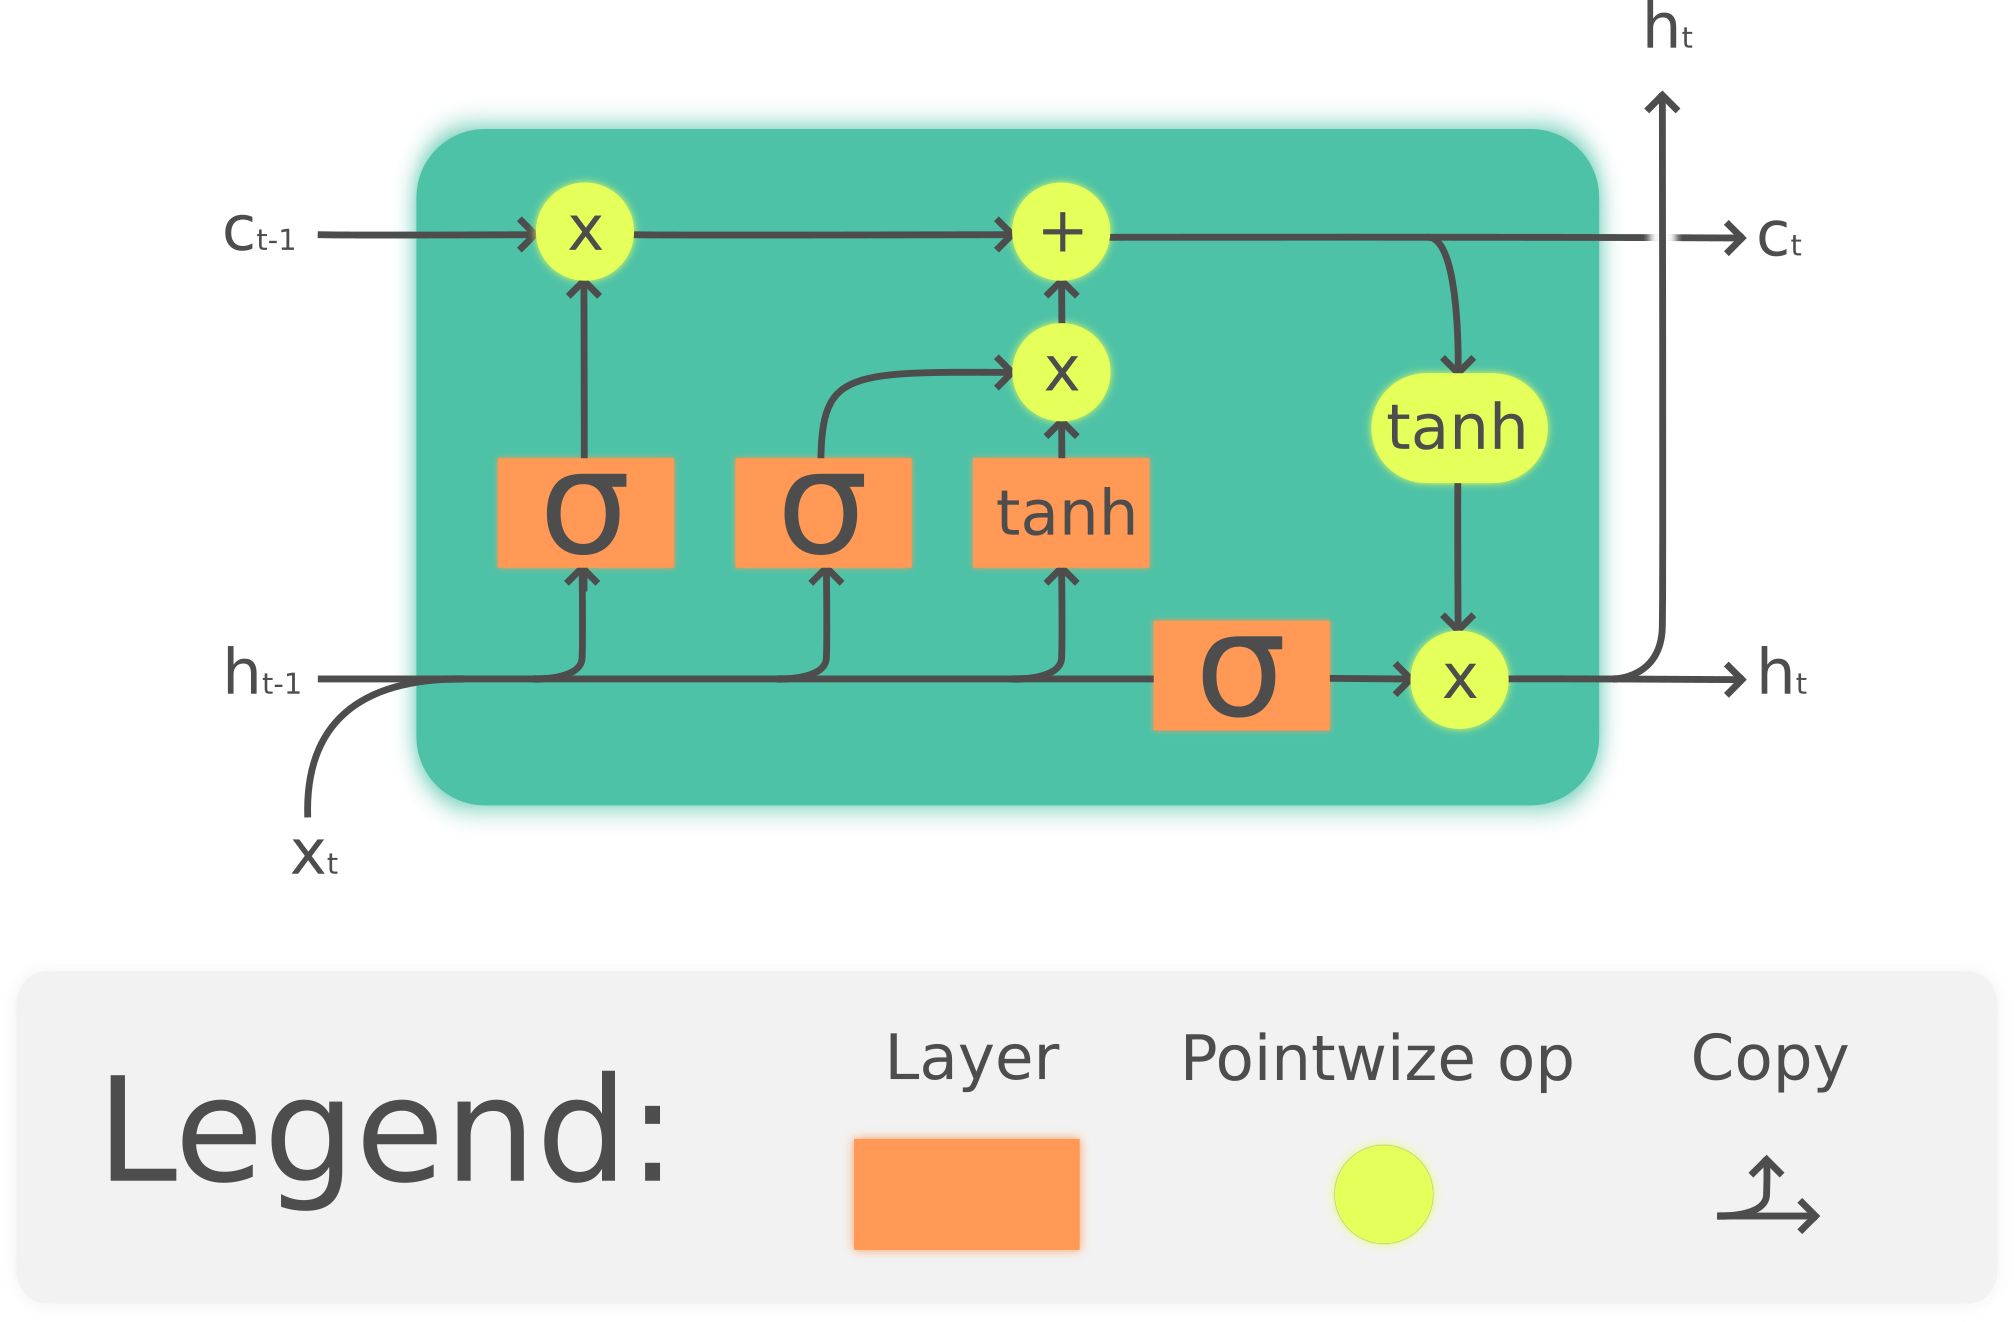
\includegraphics[width=\columnwidth]{img/computational_unit}
	\caption{The computational unit of a LSTM with input from dataset $ x(t) $, output $ h(t) $ and context function $ c(t) $. The input of the unit at time $ t $ is $ x(t)h(t-1)c(t-1) $ .}
	\label{fig:computational_unit}
\end{figure}


\begin{figure}[!h]
	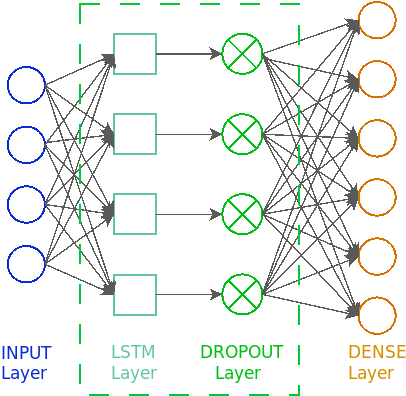
\includegraphics[width=\columnwidth]{img/LSTM}
	\caption{The general structure of the LSTM used in the experiment}
	\label{fig:LSTM}
\end{figure}
A LSTM neural network is made by at least one layer of LSTM units. The dataset to train a LSTM network in general is made by a sequence of input values and a corresponding sequence of output.
In our specific case the dataset is the time sequence of the number of infected of Covid19 in Italy. During the input preprocessing the complete sequence is divided in shorter sequences of length $ historical\_windows $ called sample. Each sample is shifted of 1 between each other and for each input sample is returned a sequence of length $ prediction\_horizon $ which represent the predicted number of infected in the next days. This two parameter are manually set and depend from external factor, such as the number of sample in the input sequence. \\ The structure of NN is as in Figure \ref{fig:LSTM}.\\ 
In Table \ref{tab:params} there are the tuned hyperparameters values chosen for the experiment. Note that the total number of possible configuration of hyperparameters is $ 12*6*8*6 = 3456 $ however as will be shown, the number of trained model will be much less, decreasing the time to find good hyperparameters.\\
\begin{table}[!h]
	\caption{Table of the values to tune for the model. The chosen value for each parameter are: number of units per layer $ L_i $, Learning Rate ($ LR $), dropout percentage ($ D $) and number of LSTM layers ($ N $). }
	\begin{tabular}{ccccc}
		   &$L_i$ &   $ LR $ 	& $D $ & $N$\\ 
	\hline
		1  & 25   & $ 10^{-1} $	& 0.05 & 1	\\
		2  & 50   & $ 10^{-2} $ & 0.10 & 2 	\\
		3  & 75   & $ 10^{-3} $ & 0.15 & 3 	\\
		4  & 100  & $ 10^{-4} $ & 0.20 & 4 	\\
		5  & 125  & $ 10^{-5} $ & 0.25 & 5 	\\
		6  & 150  & $ 10^{-6} $ & 0.30 & 6 	\\
		7  & 175  &  			& 0.35 &   	\\
		8  & 200  &  			& 0.40 &   	\\
		9  & 225  &  			&      &   	\\
		10 & 250  &  			&      &   	\\
		11 & 275  &  			&      &   	\\
		12 & 300  &  			&      &   	\\
	\end{tabular}

	\label{tab:params}
\end{table}

Let's now analyze the encoding method to obtain the individual of the genetic algorithm from the LSTM trained model. Each trained model can be identified with its training hyperparameters value, moreover there are some of them which are set in every model (fixed parameters) and other that are not (variable parameter). In Figure \ref{fig:individual} it's shown the general definition of individual of CVOA genetic algorithm. As an example, if a model is trained with $ LR = 10^{-1}, D = 0.4, N = 2, L_1 = 50, L_2 = 25 $ the corresponding individual would be represented by $ [1, 8, 2] + [2, 1] $. Note that the value inside the parenthesis are the index of the corresponding value in Table \ref{tab:params}. 

\begin{figure}
	\caption{The representation of a LSTM as individual of the GA. Learning Rate ($ LR $), Dropout ($ D $ and Number of LSTM layer ($ N $) compose the fixed part of the individual and the number of LSTM unit ($ L_i $) for each LSTM layer ($ i $) represent the variable part. Note that the "+" symbol stand for concatenation.}
	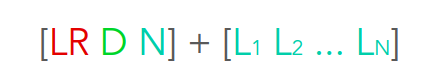
\includegraphics[width=\columnwidth]{img/individual}
	\label{fig:individual}
\end{figure}


\subsection{Genetic Algorithm}
	The genetic part of CVOA is built by following a standard Genetic Algorithm (GA) but adding and modifying some components.
The main components and functions performed by the GA are folded successively:

\subsubsection{GA Constant Parameters}
This subsection presents the main parameters used and which will be mentioned in the following sections.
All probabilities involved in the GA are based on the real data of Coronavirus propagation model.
\begin{itemize}
\item $_PDIE$: An infected individual can die with a given probability.
\item $_PSUPERSPREADER$: It is the probability that an individual spread the disease to a greater number of healthy individuals. After this condition is validated, two situations can be found: % TODO: cercare di fixare l'underscore _ che è osceno così e magari cambia il font dei nomi (senti fish)
\subitem $ORDINARY\_RATE$: It is a standard infected individual (not a super-spreader) and this rate correspondes to its infection rate
\subitem $SUPERSPREADER\_RATE$: If the infected individual turns out to be super-spreader, this is its infection rate which is at least more than double of Ordinary-Rate
\item $_PREINFECTION$: Probability that a recovered individual can be re-infected.
\item $_PISOLATION$: It corresponds to the probability of applying measures for social isolation to an individual. This parameter helps to reduce the exponential growth of the infected population after each iteration. Therefore, a high value must be assigned to this probability. Note that this value is not well defined by the real pandemic data because different countries have made different choices about it. 
\item $_PTRAVEL$: This probability simulates how an infected individual can travel to any place in the world and can infect healthy individuals.
\item $PANDEMIC\_DURATION$: This parameter simulates the duration of the pandemic.
\end{itemize}

\subsubsection{Population Individuals}
	As explained above, figure \ref{fig:individual}, the individuals of the population are composed of two arrays of integer values (fixed and variable length). They are also divided into three categories:
\begin{itemize}
\item Dead
\item Recovered
\item Infected
\end{itemize}
There is another category in which only some infected individuals can belong, according to a certain probability ($_PSUPERSPREADER$). Only individuals who have the best fitness value (MAPE) of the population have a chance to fall into this category. They are called Super-Spreaders and have a higher infection potential than other individuals. In this way the evolution of infected individuals of the following epoch will be based on individuals with good MAPE value and will be statistically better.

\subsubsection{Population}
	The population divides individuals into three different (sub)populations, managed through lists and updated and maintained during the whole algorithm, in according with the type of individuals:
\begin{itemize}
\item Dead: It contains dead individuals. They can no longer be used in the algorithm.
\item Recovered: After each epoch, infected individuals are removed from their population and inserted here. These individuals can return to influence the algorithm if they are reinfected ($_PREINFECTION$). Also individuals who simulate social distancing measures and therefore are isolated, belong to this population ($_PISOLATION$).
\item New-Infected: It holds all the new individuals that have been infected in the previous epoch.
\end{itemize}

\subsubsection{Main Steps} \label{sec:mainSteps}
\begin{itemize}
\item Patient-Zero: The initial population consists of only one individual, called patient-zero (PZ). As in the real coronavirus epidemic, it identifies the first human being infected.
\item Fitness function: The fitness function, calculated for each infected individual at each epoch corresponds to the execution of the LSTM training, which structure is specified by the hyper-parameters given by the individuals themselves.
\item Fitness Value: The fitness value of each individual is the Mean Absolute Percentage Error (MAPE) value. It is returned as a result of performing the LSTM training and tries to quantify the goodness of the hyper-parameters used, as it corresponds to the measure of the accuracy of the forecast of a forecasting method with respect to the real value.
\item Mutation: The basic process for the mutation is the single position mutation. It corresponds to the change of a value of a specific element in the fixed or variable array of an individual.
First, a signed change amount \begin{math}C \in \{-2 ,-1, +1, +2\}\end{math} is randomly determined using the following criteria. A random real number $P$ between $0$ and $1$ is generated using a uniform distribution. The change amount will be:
\begin{itemize}
\item \begin{math}C=-2 \iff P<0,25\end{math}
\item \begin{math}C=-1 \iff P<0,50\end{math}
\item \begin{math}C=+1 \iff P<0,75\end{math}
\item \begin{math}C=+2 \iff P \leq 1\end{math}
\end{itemize}
Once the amount of change is determined, the new value for the infected element is computed. If its previous value is $V$ , then the new value after the single position mutation will be \begin{math}V\textsuperscript{1} = V + C\end{math}. If the new value $V\textsuperscript{1}$ exceeds the limits defined for the individual codification, such value is set to the maximum or minimum allowed value accordingly.
%• Numerous mutations
\item Crossover: The evolution of the population, as in the real case, is not given by the reproduction of individuals, but the virus spreads from one individual to another. In this sense there is no crossover step, in its place a Propagation Function has been developed.
\item Propagation Function:
Some of the infected individuals die ($_PDIE$). Such individuals can no longer infect new individuals.
The individuals surviving the coronavirus in an epoch will infect new individuals (intensification). According to the probability $_PSUPERSPREADER$, an individual can spread the desease with two rate:
\subitem Ordinary spreader, with spreading rate given by $ORDINARY\_RATE$.
\subitem Super-spreaders, with spreading rate given by $SUPERSPREADER\_RATE$.\\
To ensure diversification, both types of spreader individuals can travel and explore solutions quite dissimilar ($_PTRAVEL$), thus allowing to propagate the disease to solutions that may be quite different. In case of not being traveler, new solutions will change according to an $ORDINARY\_RATE$.
\item Stop Criterion:
The stop criterion of this algorithm, by construction, does not need to be controlled by any parameter. The recovered and dead populations are constantly growing as time goes by, and the new infected population cannot infect new individuals. It is expected that the number of infected individuals increases for a certain number of iterations. However, from a particular iteration on, the size of the new infected population will be smaller than that of the current one because recovered and dead populations are too big, and the size of the infected population decays over time. \\
Additionally, due to time constraint, it is possible to set up a maximum number of iterations ($PANDEMIC\_DURATION$) to force the stop criterion. The social isolation measures also contributes to achieve it.
\end{itemize}

\section{CVOA Meta-heuristic}
Including the basic concepts in section \ref{basicConcepts}, it is now possible to understand the overall functioning of the CVOA and analyze it in a more specific way.
Only the most important methods will be presented. Starting with the main method of the algorithm, shown as follows:

\lstset{language=Python}
\lstset{frame=lines}
\lstset{caption={CVOA main method}}
\lstset{label={CVOAmain}}
\lstset{basicstyle=\footnotesize}
\lstset{showstringspaces=false}
\lstset{numbers=left}				
\lstset{stepnumber=1}
\begin{lstlisting}[mathescape=true]
PZ = {fixed part} + {var part}
while (PANDEMIC_DURATION $\geq$ 0 && epidemic) {
    propagateDisease()
    if (infected_population is empty)
        epidemic = false
    PANDEMIC_DURATION --
}
\end{lstlisting}
As mentioned in section \ref{mainSteps}, the initial population is composed of a single individual (PZ), with values of the arrays that compose it randomly generated (within their limits). Then a loop is performed until the stop criterion is reached. Each iteration of the cycle corresponds to an epoch of the GA, in each epoch the disease is propagated. Once the stop conditions are updated, the cycle starts again.\\
Analyzing specifically the method contained:
\subsection{propagateDisease()}
In row number 3 of Listing \ref{CVOAmain} there is the $propagateDisease()$ method. This method joins fitness evaluations, population selection, crossover and mutations functions and it is illustrated in the Pseudo-Python Code page at Listing \ref{propagateDisease}.\\
Looking inside, it is composed by several steps :
\begin{itemize}
\item Row 3: Fitness Evaluation  
\item Row 7: Update best individual
\item Row 12,16: Choose dead and super-spreader individuals
\item Row 25: Infect new individuals
\item Row 29: Looking re-infections
\item Row 33,34: Prepare populations for the next epoch.
\end{itemize}
At first, for each infected individual a $Fitness\_function$ is executed. As explained in section \ref{sec:mainSteps}, it returns values of MAPE, one for each.\\ %aggiungi LSTM
Then the infected list of individuals is sorted in increasing order by fitness (MAPE) and so, the first individual corresponds to the best and therefore the one with the lowest MAPE value. Remember that the lower the MAPE value, the more accurate the forecast with real data.
For each epoch, this individual is stored in $best\_individual$ if its fitness is lower that the current one. In this way, whenever the agorithm is stopped, the best hyper-parameters found up to now are always available.\\
The next step is to update the dead individuals and to assign the super-spreader property. Two indexes, as percentages of the infected list size, are used to divide the infected list. The infected individuals contained between $0$ to $idx\_super\_spreader$ also become super-spreaders while individuals from $idx\_deaths$ onwards die.\\
Every infected individual infects a certain number of new individuals ($nInfected$, Row 17 or 19), added to $new\_infected\_list$. The process of infection (Row 25) is described in the next section. Once the re-infections are found, the populations are updated in which the $infected$ list is added to $recovered$ list and $new\_infected\_list$ become $infected$ list. Finally the method ends.

\subsection{individual.infected(travel\_distance)}
This method, shown in Listing \ref{lnfected}, is called in Row 25 of Listing \ref{propagateDisease}. It represents the way in which an individual can infect other ones. As in the previous method, it also consists of several steps:
\begin{itemize}
\item Row 2: Infection Probability
\item Row 3: Single Position Mutation
\item Row 8: Traveler Individual
\item Row 14-23: Generation of New Infected
\end{itemize}
First of all, as mentioned earlier, there is no crossover for generating new individuals. An individual is created starting from the structure of another and applying one or more single position mutations to it. Therefore, the individual who infected a $nInfected$ new individuals calls this method $nInfected$ times. Every time, this individual is copied to a new individual ($mutated$) as a first step and then all the mutation are applied.\\
Starting from Row 2, with probability $\frac{1}{3}$, a single position mutation (section \ref{sec:mainSteps}) is applied at third value of the $fixed\_part$ array of the $mutated$ individual. If the mutation occurs, the $variable\_part$ is also resized according to the mutation value and the $_PTRAVEL$ is set to $-1$.
In this way, at Row 8, two situations are possibile:
\begin{enumerate}[label=\arabic*)]
\item $_PTRAVEL = -1$: Always if the mutation occurred or in case mutation fails but the individual who infected had a probability of $-1$ 
\item $_PTRAVEL = 1$: Because the individual who infected had a probability of $1$ and mutation fails 
\end{enumerate}
This probability determines the number of mutations applied to $mutated$.\\
From Row 14 to 23, these mutations are performed. Every mutation is a single position mutation of a random value of $fixed\_part$ or $variable\_part$ of $mutated$, except the third $fixed\_part$ value and except values that have already been changed.\\
This procedure represents the spread of the disease from one individual to another and therefore the creation of the population of infected individuals of the following epoch.

\section{Experiment Evaluation}
There are 2 different assessments to make for CVOA algorithm:
\begin{enumerate}[label=\arabic*)]
\item GA Evolution
\item Predict Accuracy
\end{enumerate}
The first, GA Evolution, is visible to the figure \ref{fig:GAgraph} which contains all the information needed to evaluate the goodness of the trend of the GA. A brief explanation of the parts that make up the figure is as follows:
\begin{itemize}
\item Top: Timer represent hours, minutes and seconds in the form HH:MM:SS
\item Top-Left: Populations counter
\item Top-Right: Best Individual found with its relative MAPE, percentage of $recovered$ on $infected$
\item Top-Center: Last current individual to whom fitness has been calculated
\item Center: Graph which relates the MAPE value of all individuals to epoches 
\end{itemize}
This image represent the evolution of GA until the tenth epoch. For each epoch (epoch $i$ is shown between the value $i-1$ and $i$ of the x axis)

\clearpage
\onecolumn
\begin{figure}[!h]
	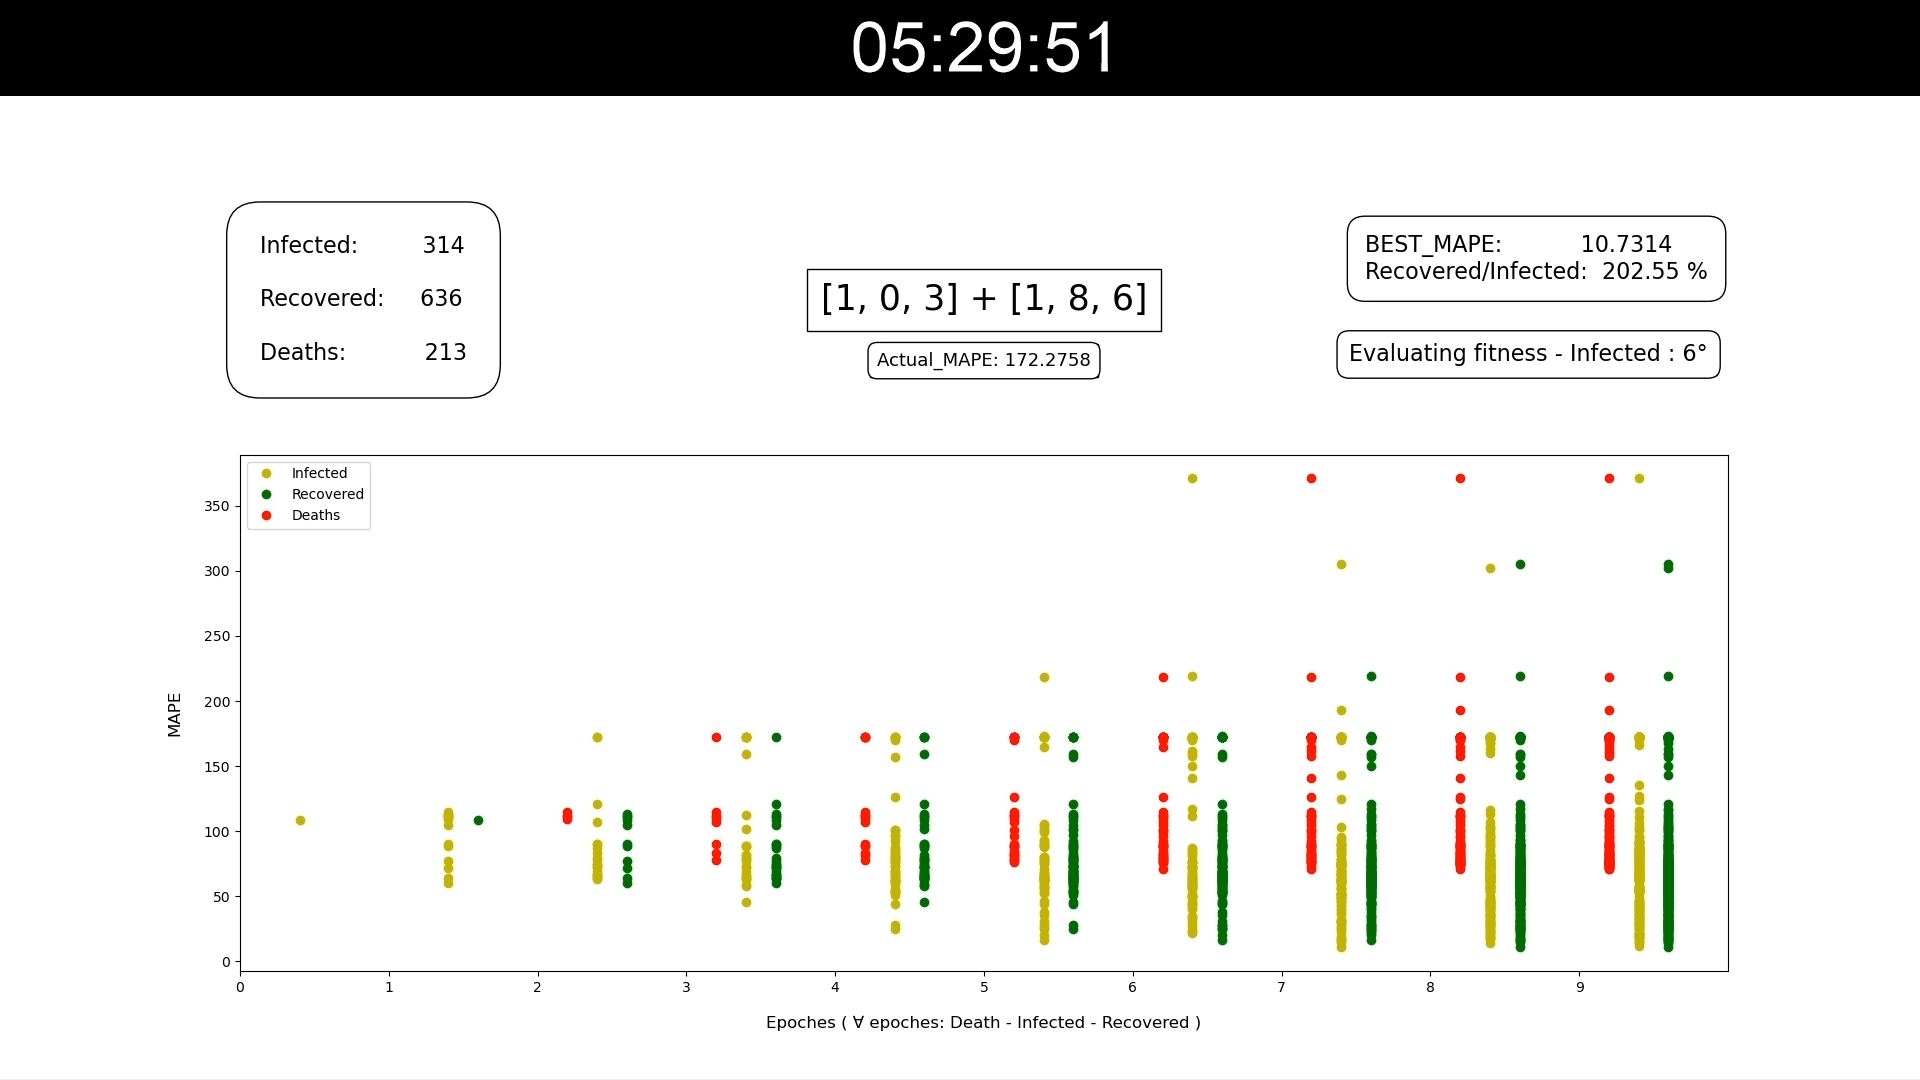
\includegraphics[width=\columnwidth]{img/GA_algorithm_iter10}
	\caption{GA trend graph}
	\label{fig:GAgraph}
\end{figure}

\begin{table}[!h]
	\caption{Table result....}
	\begin{tabular}{cccccccccccccccc}
		   &$AU$&$A$&$BE$&$CA$&$FL$&$F$&$D$&$IN$&$IT$&$NY$&$RU$&$ES$&$UK$&$US$&$WA$\\
	\hline
		Australia (AU) &  &  &  &  &  &  &  &  &  &  &  &  &  & \\
		Austria (A) &  &  &  &  &  &  &  &  &  &  &  &  &  & \\
		Belgium (BE) &  &  &  &  &  &  &  &  &  &  &  &  &  & \\
		California (CA) &  &  &  &  &  &  &  &  &  &  &  &  &  & \\
		Florida (FL) &  &  &  &  &  &  &  &  &  &  &  &  &  & \\
		France (F) &  &  &  &  &  &  &  &  &  &  &  &  &  & \\
		Germany (D) &  &  &  &  &  &  &  &  &  &  &  &  &  & \\
		India (IN) &  &  &  &  &  &  &  &  &  &  &  &  &  & \\
		Italy (IT) &  &  &  &  &  &  &  &  &  &  &  &  &  & \\
		NewYork (NY) &  &  &  &  &  &  &  &  &  &  &  &  &  & \\
		Russia (RU) &  &  &  &  &  &  &  &  &  &  &  &  &  & \\
		Spain (ES) &  &  &  &  &  &  &  &  &  &  &  &  &  & \\
		UK &  &  &  &  &  &  &  &  &  &  &  &  &  & \\
		US &  &  &  &  &  &  &  &  &  &  &  &  &  & \\
		Washington (WA) &  &  &  &  &  &  &  &  &  &  &  &  &  & \\
	\end{tabular}

	\label{tab:params}
\end{table}
\clearpage
\twocolumn

\section{Conclusion}
In this report it was analyzed the CVOA metaheuristic which automatically estimate some good value for the hyperparameter for a ML algorithm. As seen there are two main advantages:
\begin{itemize}
	\item the hyperparameter of the GA are that known from the coronavirus, preventing from tuning them manually;
	\item the algorithm automatically terminate after certain number of iterations,
	\item the metaheuristic automatically adapt on the context of the ML problem, indeed it could be used either in machine vision or in data sequence forecasting.
\end{itemize}
Ad disadvantage, the number of infected in the first iterations is exponential and the execution time is still high.

\subsection{Future Work}
One of the possible improvement of the algorithm is to reduce the number of infected considering the metaphor of the production of a vaccine. This could be done by adding a percentage of  \textit{VACCINATED\_INDIVIDUAL} .\\
Moreover, an open-source library would simplify the implementation of the CVOA algorithm. The NN model could be passed as parameter, with a method to determine the GA individual from the model and with the fitness function.\\
Covid-19 has an high level of mutation such as there are spreading different type of virus. A parallel version of multi-covid CVOA could be implemented where the infected and the recovered are shared among all the viruses but all of them has different probability of infection and death. 
\clearpage
\onecolumn
\section{Pseudo-Python Code}
\lstset{language=Python}
\lstset{frame=lines}
\lstset{caption={propagateDisease method}}
\lstset{label={propagateDisease}}
\lstset{basicstyle=\footnotesize}
\lstset{showstringspaces=false}
\lstset{numbers=left}					% show row number (to use them in code?)
\lstset{stepnumber=1}
\begin{lstlisting}[mathescape=true]
new_infected_list = []
for (individual in infected_population):
    individual.fitness = fitness_function(individual)

infected_population = sorted(infected, key=lambda i: i.fitness)
if(best_solution.fitness > infected_population[0].fitness):
    best_solution = infected_population[0]
idx_super_spreader = S$\textsubscript{\%}$ * len(infected_population)
idx_deaths = D$\textsubscript{\%}$ * len(infected_population)

for (individual in infected_population):
    if (idx_individual $\geq$ idx_deaths):
        infected_population.remove(individual)
        dead_population.add(individual)
    else:
        if (idx_individual < idx_super_spreader):
            nInfected = MIN_SUPERSPREAD + random.randint(0, MAX_SUPERSPREAD - MIN_SUPERSPREAD)
        else:
            nInfected = random.randint(0, MAX_SPREAD)
            if (individual is traveler):
                traverl_distance = -1
            else: 
                traverl_distance = 1
        while (nInfected > 0):
            new_infected = individual.infect(travel_distance)
            if (new_infected $\notin$ dead_population || 
                                infected_population || new_infected_list || recovered_population): 
                new_infected_list.add(new_infected)
            if (new_infected $\in$ recovered_population && new_infected $\notin$ new_infected_list): 
                if (random.random() < $_PREINFECTION$): 
                    new_infected_list.add(new_infected)
                    recovered_population.remove(new_infected)
            nInfected --
        recovered_population.add(infected) 
        infected_population = new_infected_list
\end{lstlisting}
\lstset{language=Python}
\lstset{frame=lines}
\lstset{caption={individual.infected(travel\_distance) method}}
\lstset{label={lnfected}}
\lstset{basicstyle=\footnotesize}
\lstset{showstringspaces=false}
\lstset{numbers=left}				
\lstset{stepnumber=1}
\begin{lstlisting}[mathescape=true]
mutated = deepcopy(individual)
if (random.randin(0, 2) == 0)
    value = mutated.single_position_mutation(individual.fixed_pard[2])
    mutated.var_part.resize(value)
    travel_distance = -1 

total_size = len(mutated.fixed_part) + len(mutated.var_part) 
if (travel_distance < 0): 
    nMutated = random.randint (0, total_size-1)
else: 
    nMutated = 1
count = 0
mutated_positions = []
while (count < nMutated):
    pos = random.randint(0, total_size-1)
    if (pos $\notin$ mutated_positions && pos $\neq$ 2)
        if (pos < mutated.fixed_part - 1):
            max_value, min_value = MAX_VAL_FIXED_PART, MIN_VAL_FIXED_PART
        else:
            max_value, min_value = MAX_VAL_VAR_PART, MIN_VAL_VAR_PART
        mutated_position[pos] = random.randint(min_value, max_value)

    count ++
\end{lstlisting}
\clearpage
\twocolumn

\printbibliography

\end{document}
